\section{Ionic Liquid Gating Experiments on Topological Insulators}
\label{sec:liquid:gating}

\subsection{Background and Introduction}

As explained in the above chapters, Bi$_2$Te$_2$Se has one of the most insulating bulk among all the Bi-based topological compounds, and its high-mobility surface state has been detected by quantum oscillations in transport experiments even at a temperature as high as 38 K~\cite{Xiong2012}. However, the surface chemical potential $E_F$ in our as-grown Bi$_2$Te$_2$Se crystals is persistently quite high ($\sim$200 meV above the Dirac Point), despite the large amount of effort that we have taken to bring down the chemical potential by the chemical doping method. Since the chemical doping method often changes the carrier density by a large amount, the chemical potential is easily tuned outside the bulk band gap. Furthermore, it is common that different segments of the as-grown Bi-based TI crystals have different $E_F$, adding the difficulty in the transport study. Thus it is desirable to tune the $E_F$ by an \emph{in-situ} gating method in order to explore the Dirac point. 

%Many groups have applied conventional electrostatic gating to tune the chemical potential $E_F$ both in exfoliated crystals~\cite{Check11,Pablo,Morpurgo} and in thin-film samples of Bi$_2$Se$_3$.~\cite{Steinberg}. Also, almost simultaneously with us, some groups started to leverage the newer technique, namely liquid gating method, to change the $E_F$ of Bi-based materials~\cite{Iwasa,Fuhrer,Check12,Iwasa12,Ando12}. These groups have shown a powerful gating ability on TI that the ionic liquid could have. However, in those work, the crucial surface quantum oscillations were absent, and the properties of the surface Dirac electrons at different $E_F$ remain to be explored.

%In our experiment, we immerse the 50um thick Bi$_2$Te$_2$Se samples with the gold-wired contacts in the ionic liquid DEME-TFSI, comprised of cations (CH$_3$ CH$_2$ )$_2$ (CH$_2$ CH$_2$ OCH$_3$ )CH$_3$ N+ and anions (CF$_3$SO$_2$)$_2$N?. The crystal dimensions of Sample 1 are 0.9?0.75? 0.05 mm$^3$. For Sample 2, they are 1.35 ? 0.61 ? 0.026 mm$^3$. The liquid is first pumped at $25 \,^{\circ}{\rm C}$ for 2 h prior to application in order to minimize any water content. Then the sample, the ionic liquid and the gold gate plate are put into a sapphire container, and are quickly loaded into the cryostat. Then the sample is fast cooled down to around 220K to reduce any chemical reaction or damage that could happen to the sample before the liquid freezes. After the gate voltage $V_G$ is applied to the gold plate at a �gating temperature� around 220K(see below), the sample is cooled to 4 K slowly (at 2K/min) to reduce the stress on the sample caused by the freezing ionic liquid. At 4 K, the large $E$-field induced by the frozen surface anion density $N_{ion}$ (1-4$\times 10^{14}$ cm$^{-2}$) creates a depletion layer that penetrates deep into the bulk (5-20 $\mu$m) (We will provide the analysis in later sections). As shown in Fig. \ref{figRRH}b (inset), the induced upward bending of the bands decreases $E_F$.This cooling process has a possibility to damage the sample as we find that repeated freezing and thawing of the ionic liquid can snap the leads or the crystal itself. Also, a large |$V_G$| may trigger an electrical discharge which invariably leads to a steep collapse of R (at 5 K).
%
%Unlike in thin films, changes to the resistance of our bulk samples caused by |$V_G$| are not resolved above ?100 K [see Fig. \ref{figRRH}], possibly due to their thickness and large amount of thermally activated carriers at high temperatures. As previous ionic liquid gating experiments (citations), every time we change $V_G$, we need to warm up the sample to the "gating temperature" around 220K and change $V_G$ by small steps. At the "gating temperature", a typical way to change $V_G$ is to change it in steps of ?0.02 V, while monitoring the transient current $I_trans$ (1-40 nA). The time spent at the "gating temperature" is typically 300�500 s, as we will discuss later in this chapter. Then the sample is cooled down to 5K slowly with the gating voltage fixed. To minimize the sample damage, we start at $V_G$ = 0 during the first cool-down, followed by measurements at increasingly negative $V_G$ until the sample fails (usually by a discharge event).  We emphasize that the changes to ? and nH are reversible (see below) as long as |$V_G$| does not exceed a limit. Upon returning $V_G$ to 0, we could recover the same starting value of R (at 5 K) provided |$V_G$|  is kept below 2 V.

%%%%%%%%%%%%%%%%%%%%%%%%%%%%%%%%%%
%%%%%%%%%%%%%%%%%%%%%%%%%%%%%%%%%%
%%%%%%%%%%%%%%%%%%%%%%%%%%%%%%%%%% FIGURE 1

%%%%%%%%%%%%%%%%%%%%%%


In this chapter, we will discuss our ionic liquid gating experiments on Bi$_2$Te$_2$Se. We observed prominent Shubnikov-de Haas oscillations in our magneto-resistance measurement at various gating voltages. Our results show that the periods of  the surface SdH oscillations can be changed over a broad range by an ionic liquid called DEME-TFSI. We find that ionic liquid could reduce $E_F$ by 50\% and we are able to access the $N$ = 1 Landau level in a magnetic field $B$ = 14 T. It allows us to investigate Bi$_2$Te$_2$Se's $\pi$ Berry phase with greatly improved resolution, as the $\frac12$-shift in the index plot remains fixed when the surface chemical potential is brought down by 50\%. More importantly, one surprising finding is that our ionic liquid gating method enhanced the surface mobility $\mu_s$ by three times according to our enlarged quantum oscillations. A possible explanation is the "smoothing" of the local potential fluctuations that increase the scattering of the surface electrons. The ionic liquid gating method provides us an opportunity to explore the direct information of both the bulk and surface with different chemical potentials, such as how the surface and bulk mobilities change with the gate voltage $V_G$. 

To fully understand the change of the surface and bulk carrier densities as well as the band bending effect in our gating experiment, we also combine the inferred parameters from the quantum oscillations and a semiclassical two-band model to explain Bi$_2$Te$_2$Se's Hall signals under different gating voltages. From the clear and large SdH oscillation data, we can obtain five transport parameters at each $V_G$, including the chemical potential $E_F$ and the mobility $\mu_s$ of the surface carriers, the bulk density and mobility, and the total ionic charge Q deposited on the surface of the sample. These five parameters together provide us a comprehensive and detailed picture of our gating experiments and the band-bending model. Also, since the parameters inferred from the SdH oscillations typically have very small error bars, such test greatly reduces the possibility for misunderstanding the experimental data. Through these analysis, we could also determine the depletion capacitance C$_d$ as well, which measures the polarizability of the depletion region.


%Despite the strong gate tuning ability of ionic liquid, there is some debate on whether the change of $E_F$ is caused by its large capacitance or by chemical reactions. To fully understand the mechanism behind, we discuss our evidence that the liquid gating in our experiment is inducing band bending rather than unwanted chemical reaction. 
\subsection{Experimental Details}





%The crystal dimensions of Sample 1 are 0.9?0.75? 0.05 mm$^3$. For Sample 2, they are 1.35 ? 0.61 ? 0.026 mm$^3$. In Sample 2, the steepest change in ?s occurs between $V_G$ = 0 and $V_G$ =?1.5V,at which $\mu_s$ =2800 $cm^2/Vs$.At a larger gate, it saturates ($\mu_s$ = 3000 $cm^2/Vs$ at ?6 V).

In our gating experiments, we follow the steps introduced in the previous chapter ``Experimental Setup'' to tune the gating voltages, and are able to change the sample's longitudinal and Hall resistance by a significant amount. The change of the sample resistance can be seen clearly in the resistance-temperature curves as displayed in Fig. \ref{figRRH}. As reported earlier~\cite{Ando10,Xiong2012,Xiong2012b}, the resistance $R(T)$ of $n$-type as-grown Bi$_2$Te$_2$Se rises dramatically to very large values as $T\to$ 4 K (curve at $V_G$ = 0 in Fig. \ref{figRRH}a). As a negative $V_G$ is added to the sample, the 4 K resistance increases as $|V_G|$ becomes larger, and eventually is enhanced by 40$\%$ at the most negative $V_G$ (Fig. \ref{figRRH}a). Previous work on the Hall coefficient has shown that at 5 K the population of bulk $n$-type carriers is much higher than the population of surface electrons (Fig. \ref{figRRH}b). Through the ionic liquid gating, the Hall coefficient $|R_H|$ increases by a factor of 2 at 5 K (Panel b) at the largest $|V_G|$. But at $|V_G| >$ 3 V both R and $R_H$ saturate, as expected for the ionic liquid gating experiments\cite{Yuan2011}. Previous work shows that chemical reactions start to happen at these voltages\cite{Yuan2011}. The change in both the resistance and the Hall coefficient at different $V_G$ suggests an upward bending of the bands and a decrease of $E_F$ at negative $V_G$ as long as $V_G$ does not exceed the depletion limit.

%The chemical doping to the sample in a strong $\bf E$ field is an an important concern in liquid-gating experiments. 

\begin{figure}[!htbp]
  \begin{center}
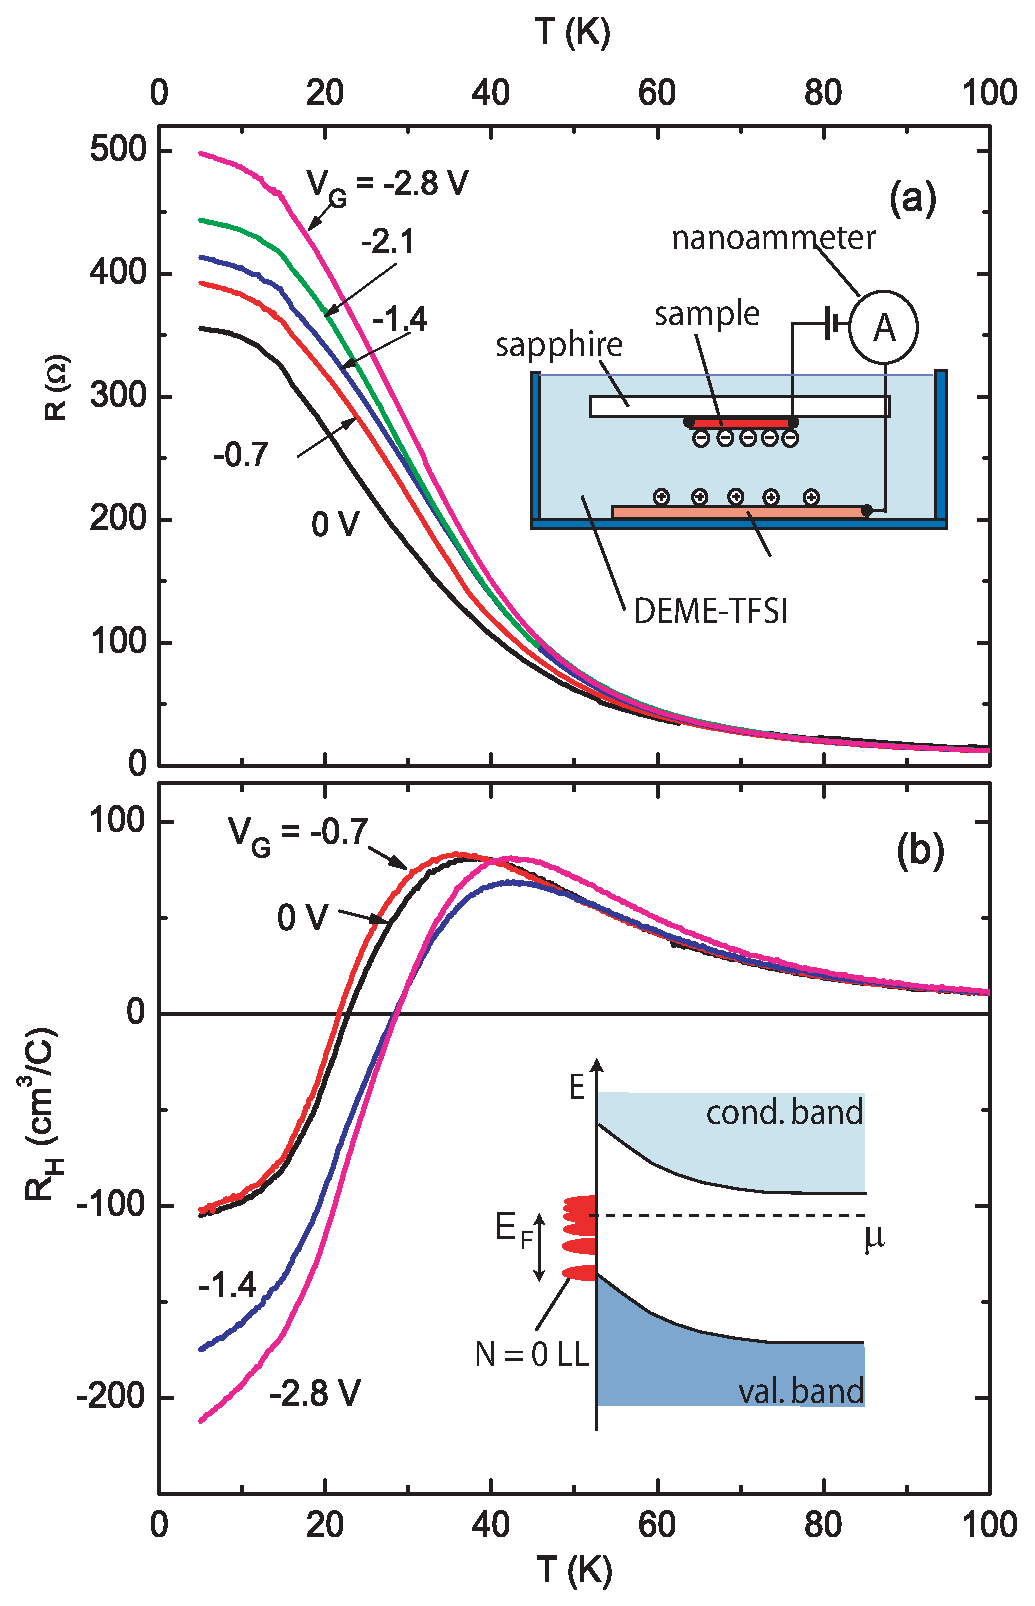
\includegraphics[width=0.75\linewidth]{ch-liquid/figures/FigRR.eps}
\caption{\label{figRRH} The resistance $R$ per square (Panel a) and
Hall coefficient $R_H$ vs. $T$ (Panel b) in Bi$_2$Te$_2$Se at selected $V_G$ in Sample 1. 
$R_H$ is measured at fixed $B$ (3 T) using the reciprocal method in Ref. \cite{Sample1987}. When $V_G$ is changed from 0 to -2.8 V, $R$ increases by 40$\%$ and $|R_H|$ increases by 2$\times$ around 5 K. The inset (Panel a) shows 
the cell housing the sample and the ionic liquid DEME-TFSI. The Au gate electrode (a
circular plate of radius 1.5 mm) is separated by 0.5 mm from the sample.
The inset in (b) is a sketch of the band bending induced by liquid gating. 
Negative ions deposited on the crystal leads to upward band-bending and a decrease of surface chemical potential towards the Dirac point. Landau levels formed by the surface electrons are shown as solid half-ovals.
}
  \end{center}
\end{figure}


Though the ionic liquid appears to have a strong power to change the carrier density in the sample, there is a debate about whether such a change is caused by its large capacitance or by certain chemical reactions. To investigate this issue, we set up some measurement in which $V_G$ is reversed, as we will discuss in the appendix. Briefly speaking, we notice that any changes caused by chemical reactions are inherently nonreversible. It means that if the chemical doping is the main reason for the changes in $\rho$ and $n_H$ at finite $V_G$, then the values of $\rho$ and $n_H$ should not return to their starting values by resetting $V_G$ to 0 V, as the chemical damage to the sample could not be recovered. And we can examine such changes at 4 K as the changes in $\rho$ and $n_H$ are most distinct at 4K. Therefore, by cycling $V_G$ we will be able to tell whether severe chemical doping has happened to the sample or not. If the band bending is the dominant effect in our gating experiment and chemical reaction effects are minimal, there will be no hystereses in $\rho$ and $n_H$ (measured at 4 K) as $V_G$ is cycled. Otherwise, we should be able to notice a large hysteresis. Thus we need to test the absence of resolvable hystereses in $\rho$ and $n_H$ when cycling the gating voltages. In addition, the test can tell us the voltage limit under which the chemical reactions can be neglected. We will show the results of such tests in the appendix. To introduce it briefly, we performed many tests on Sample 3 to investigate details of the ion accumulation in the $V_G$ cycling process over a broad range of gating temperatures (208 $<$ T $<$ 260 K). We have not performed these tests on Samples 1 and 2, from which the detailed SdH results were obtained, as we hope to minimize stress damage to their surfaces.

\begin{figure}[!htbp]
  \begin{center}
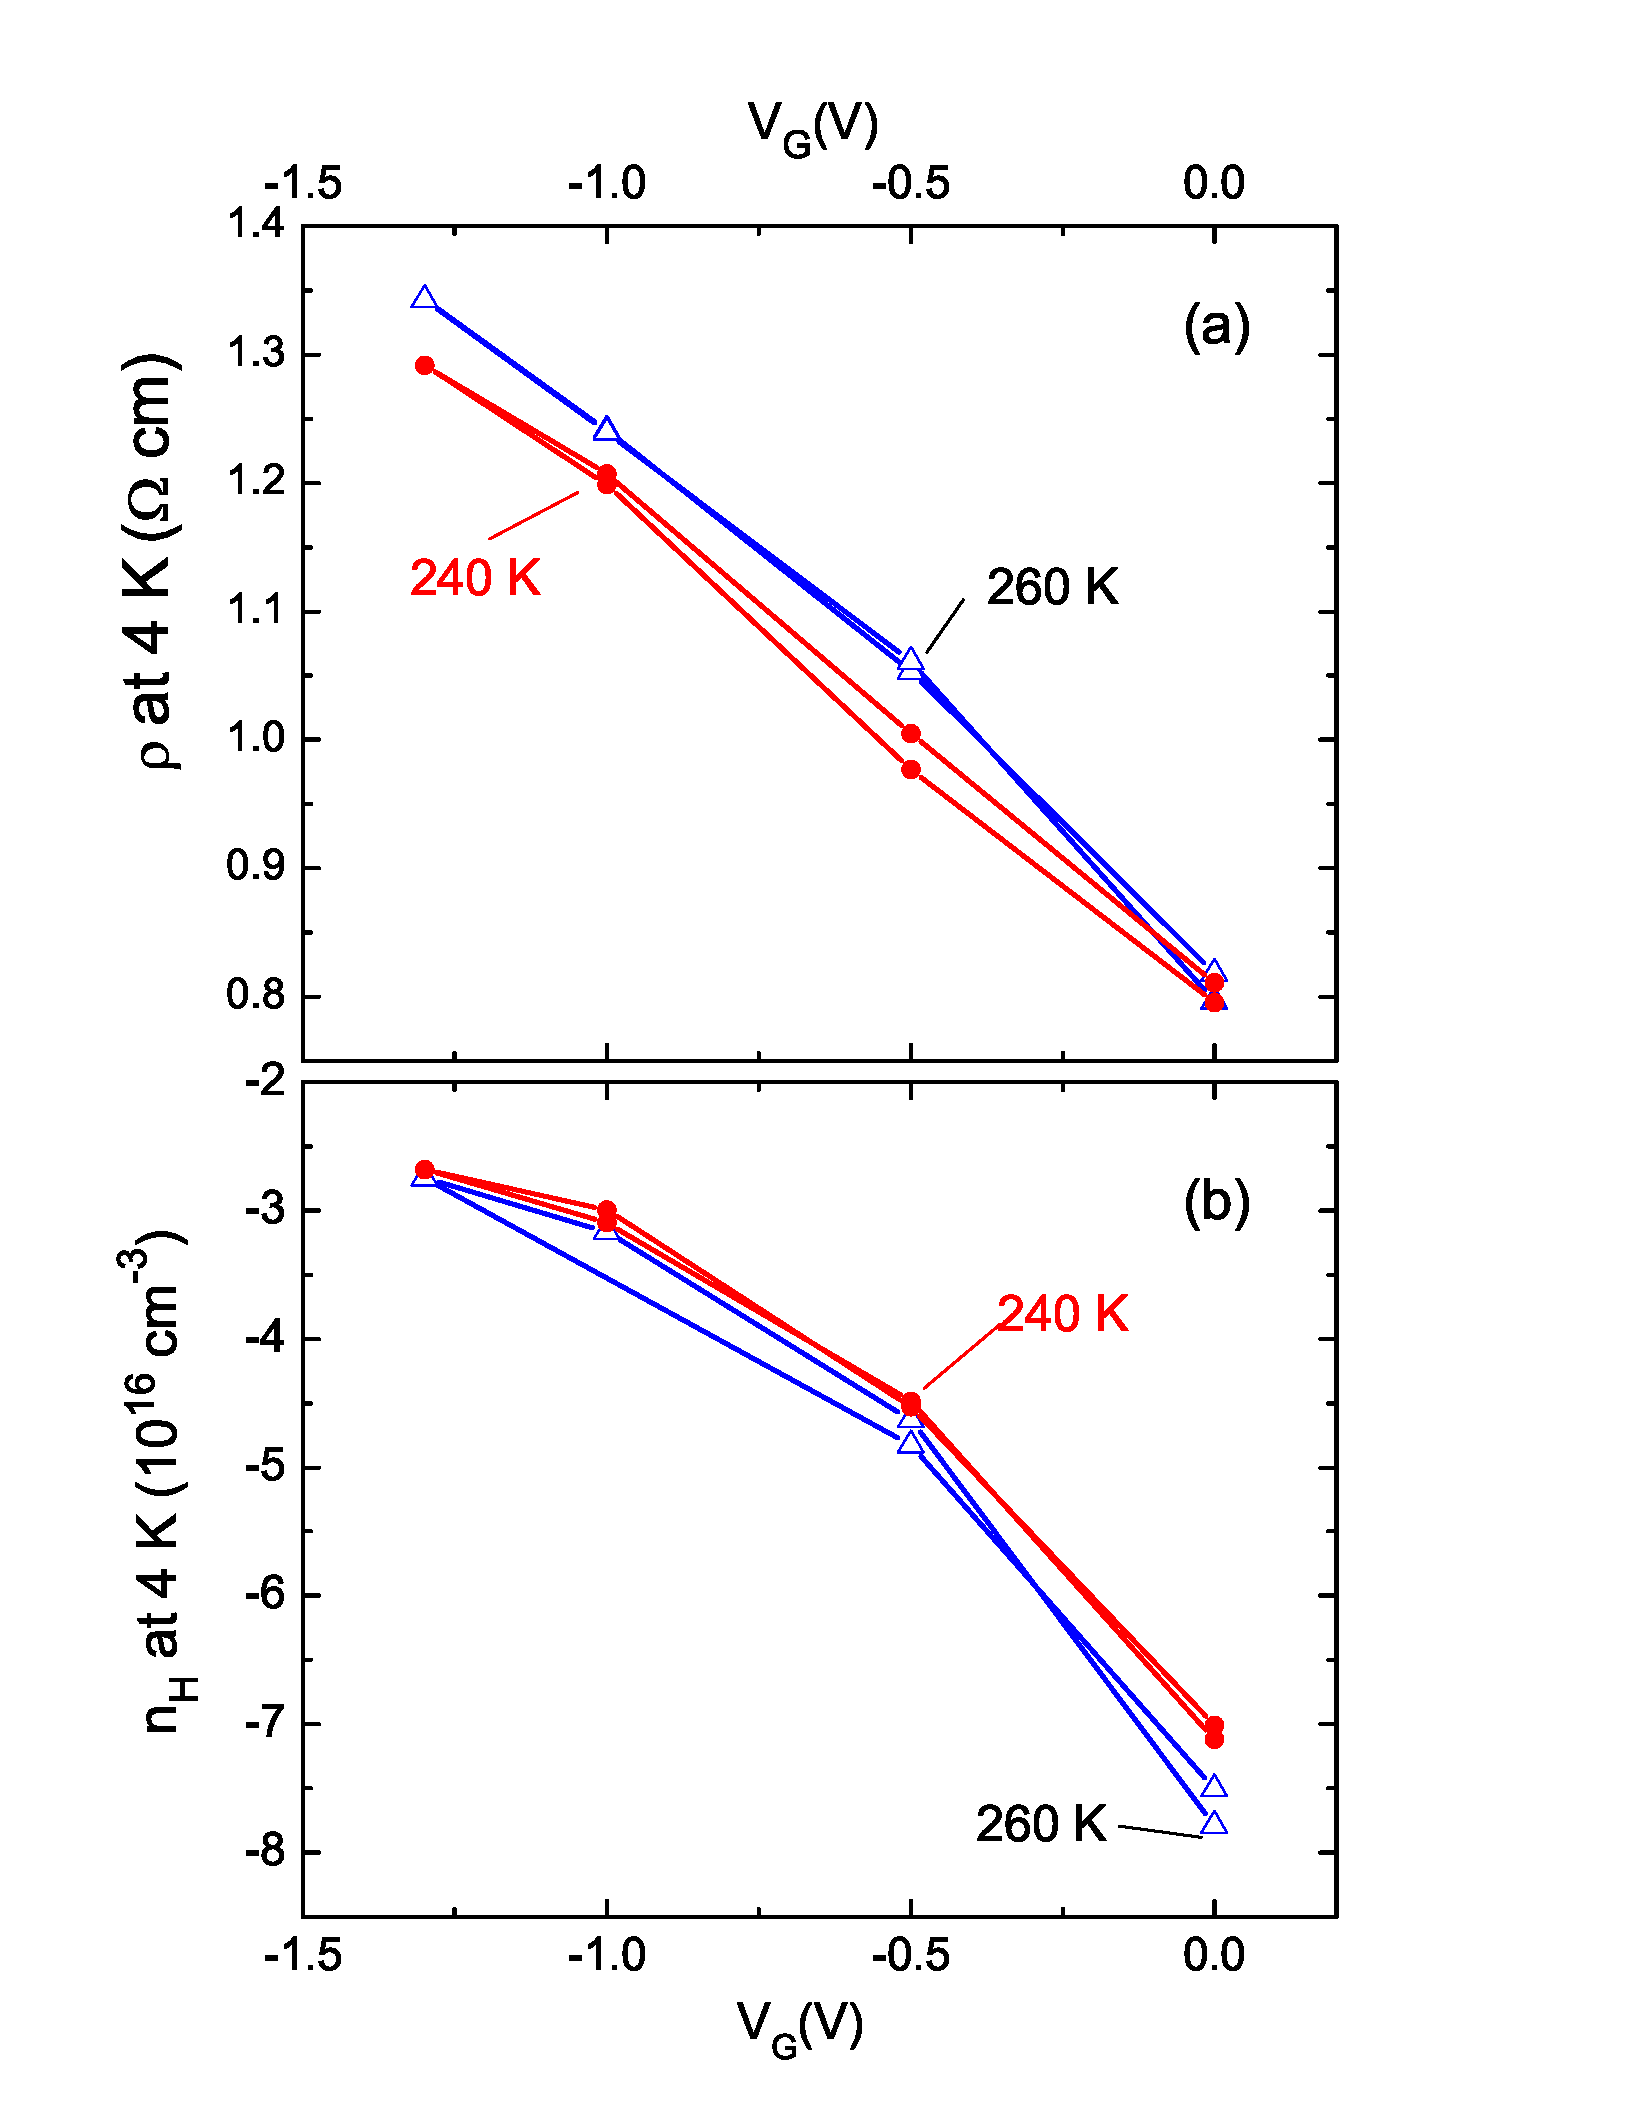
\includegraphics[width=0.75\linewidth]{ch-liquid/figures/FigRvsVG.eps}
\caption{\label{RvsVG} 
Test experiments to show negligible hysteresis in the sample�s resistivity $\rho$ (a) and Hall density $n_H$ (b), as $V_G$ is changed from 0 to -1.3 V, then back to 0 V at temperatures T = 240 and 260 K (Sample 3). The small hysteresis (within the measurement uncertainties) is taken as evidence that the chemical reaction is negligible compared with the physical gating effect. The accumulation time is 800 s in order to collect all the charge.
}
  \end{center}
\end{figure}


Fig. \ref{RvsVG} shows the main result of the $V_G$ cycling experiment on Sample 3. $V_G$ is changed stepwise from 0 to $-$1.3 V and back, while both $\rho$ and $n_H$ at 4 K are monitored at each step. Here $V_G$ is set anew (at the gating T = 240 K and 260 K respectively), and we wait for 800 s to accumulate all the anions before cooling to 4 K for the measurements of $\rho$ and $n_H$. During the change of $V_G$ at 240 K, we also record the transient charging current $I_{trans}$ in order to test whether the accumulated charges are fully reversible and hence cause the band-bending effects. As shown in Fig. \ref{RvsVG}, both at the gating temperature of 240 K and 260 K, $\rho$ and $n_H$ show clear variations at different $V_G$, but they have negligible hysteresis.


Apart from chemical reaction, two other important factors are incomplete melting of the ionic charge configuration when T is too close to the glass transition and the intrinsic (activated) bulk conductance of the ionic liquid. We have investigated these additional factors by measuring the charge accumulation during the $V_G$ change. We discuss them in the appendix. The detailed discussion about the choice of gating temperatures will also be in the appendix.

 
%\begin{figure}[htb]
%  \begin{center}
%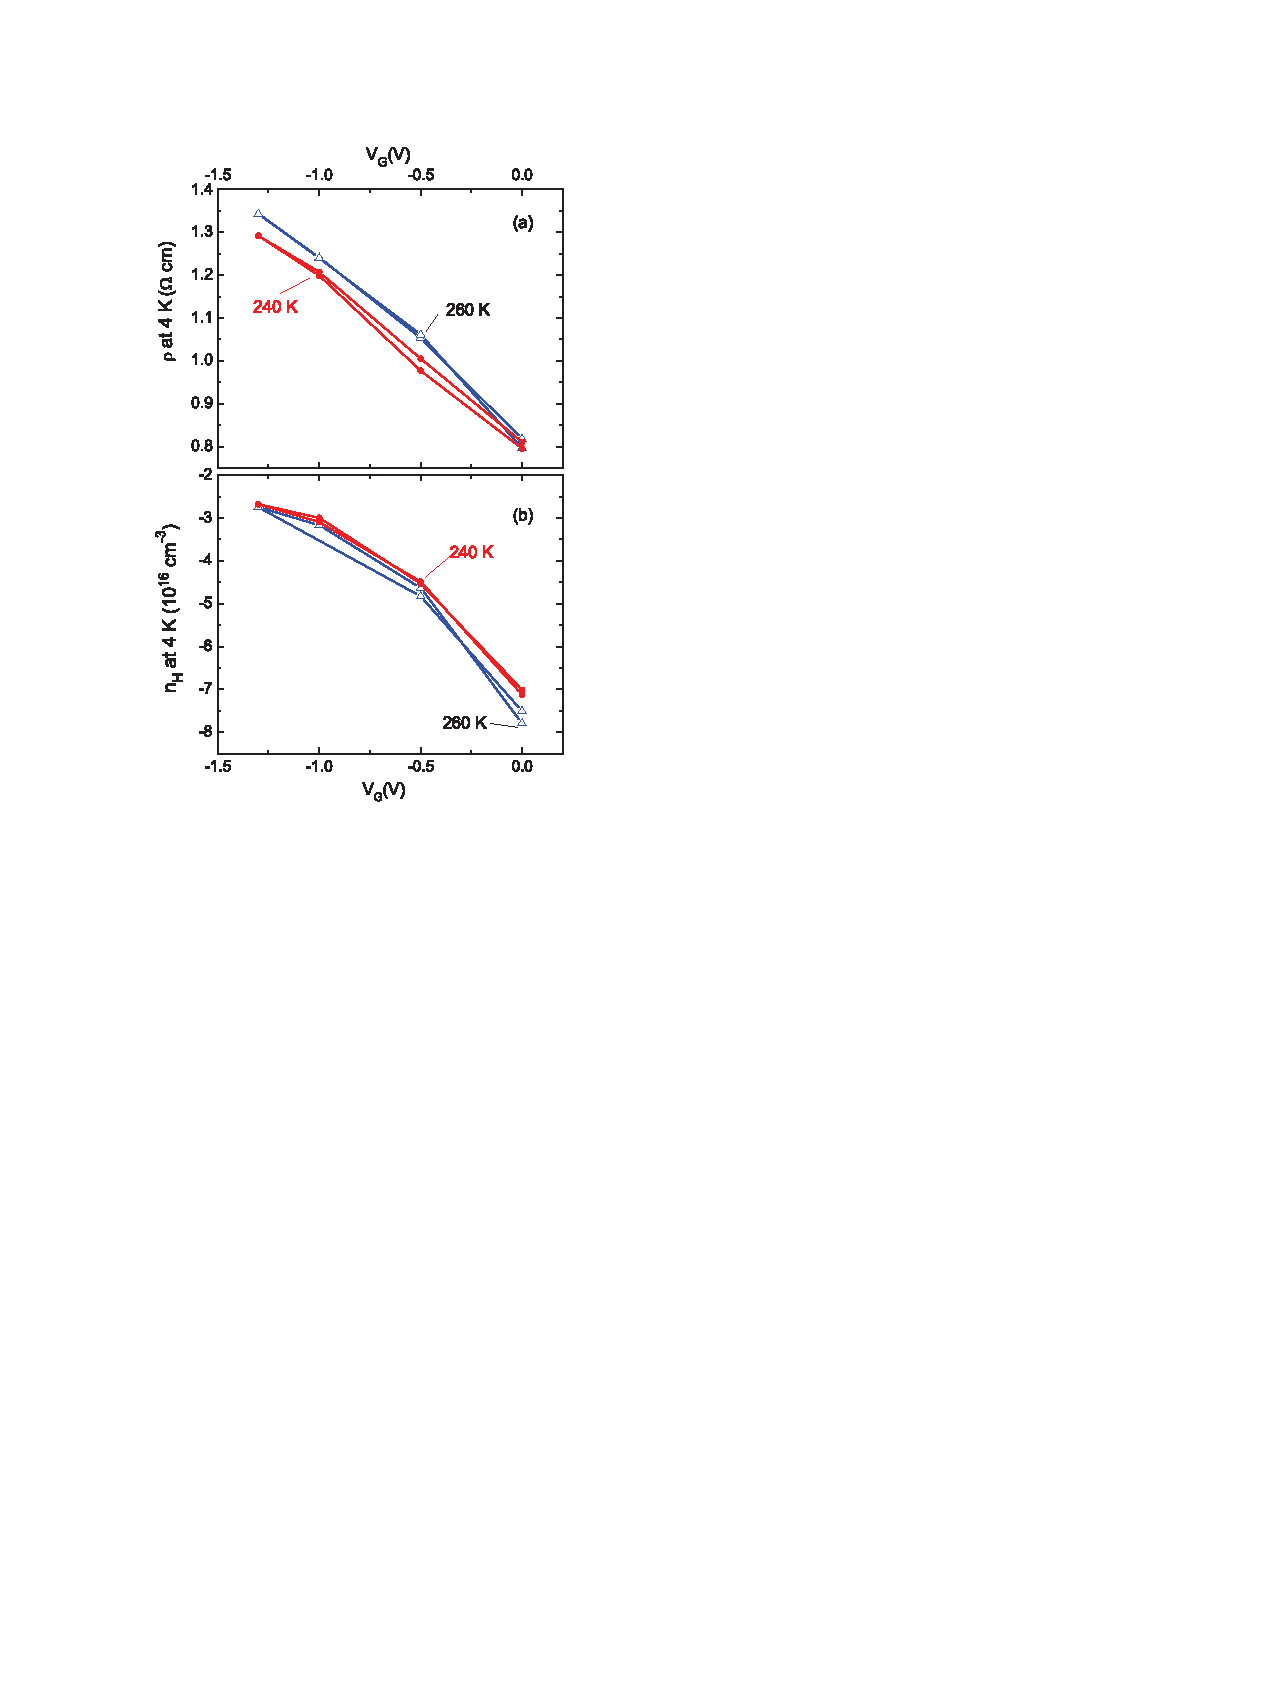
\includegraphics[width=0.9\linewidth]{ch-liquid/figures/nVg.pdf}
%\caption{\label{fignVg} (color online)
%Test experiments
%  \end{center}
%\end{figure} 

%%%%%%%%%%%%%%%%%%%%%%%%%%%%%%%%%%
%%%%%%%%%%%%%%%%%%%%%%%%%%%%%%%%%%
%%%%%%%%%%%%%%%%%%%%%%%%%%%%%%%%%% FIGURE 2


\subsection{Quantum Oscillations in Magnetoresistance under Different $V_G$}

\begin{figure}[!htbp]
  \begin{center}
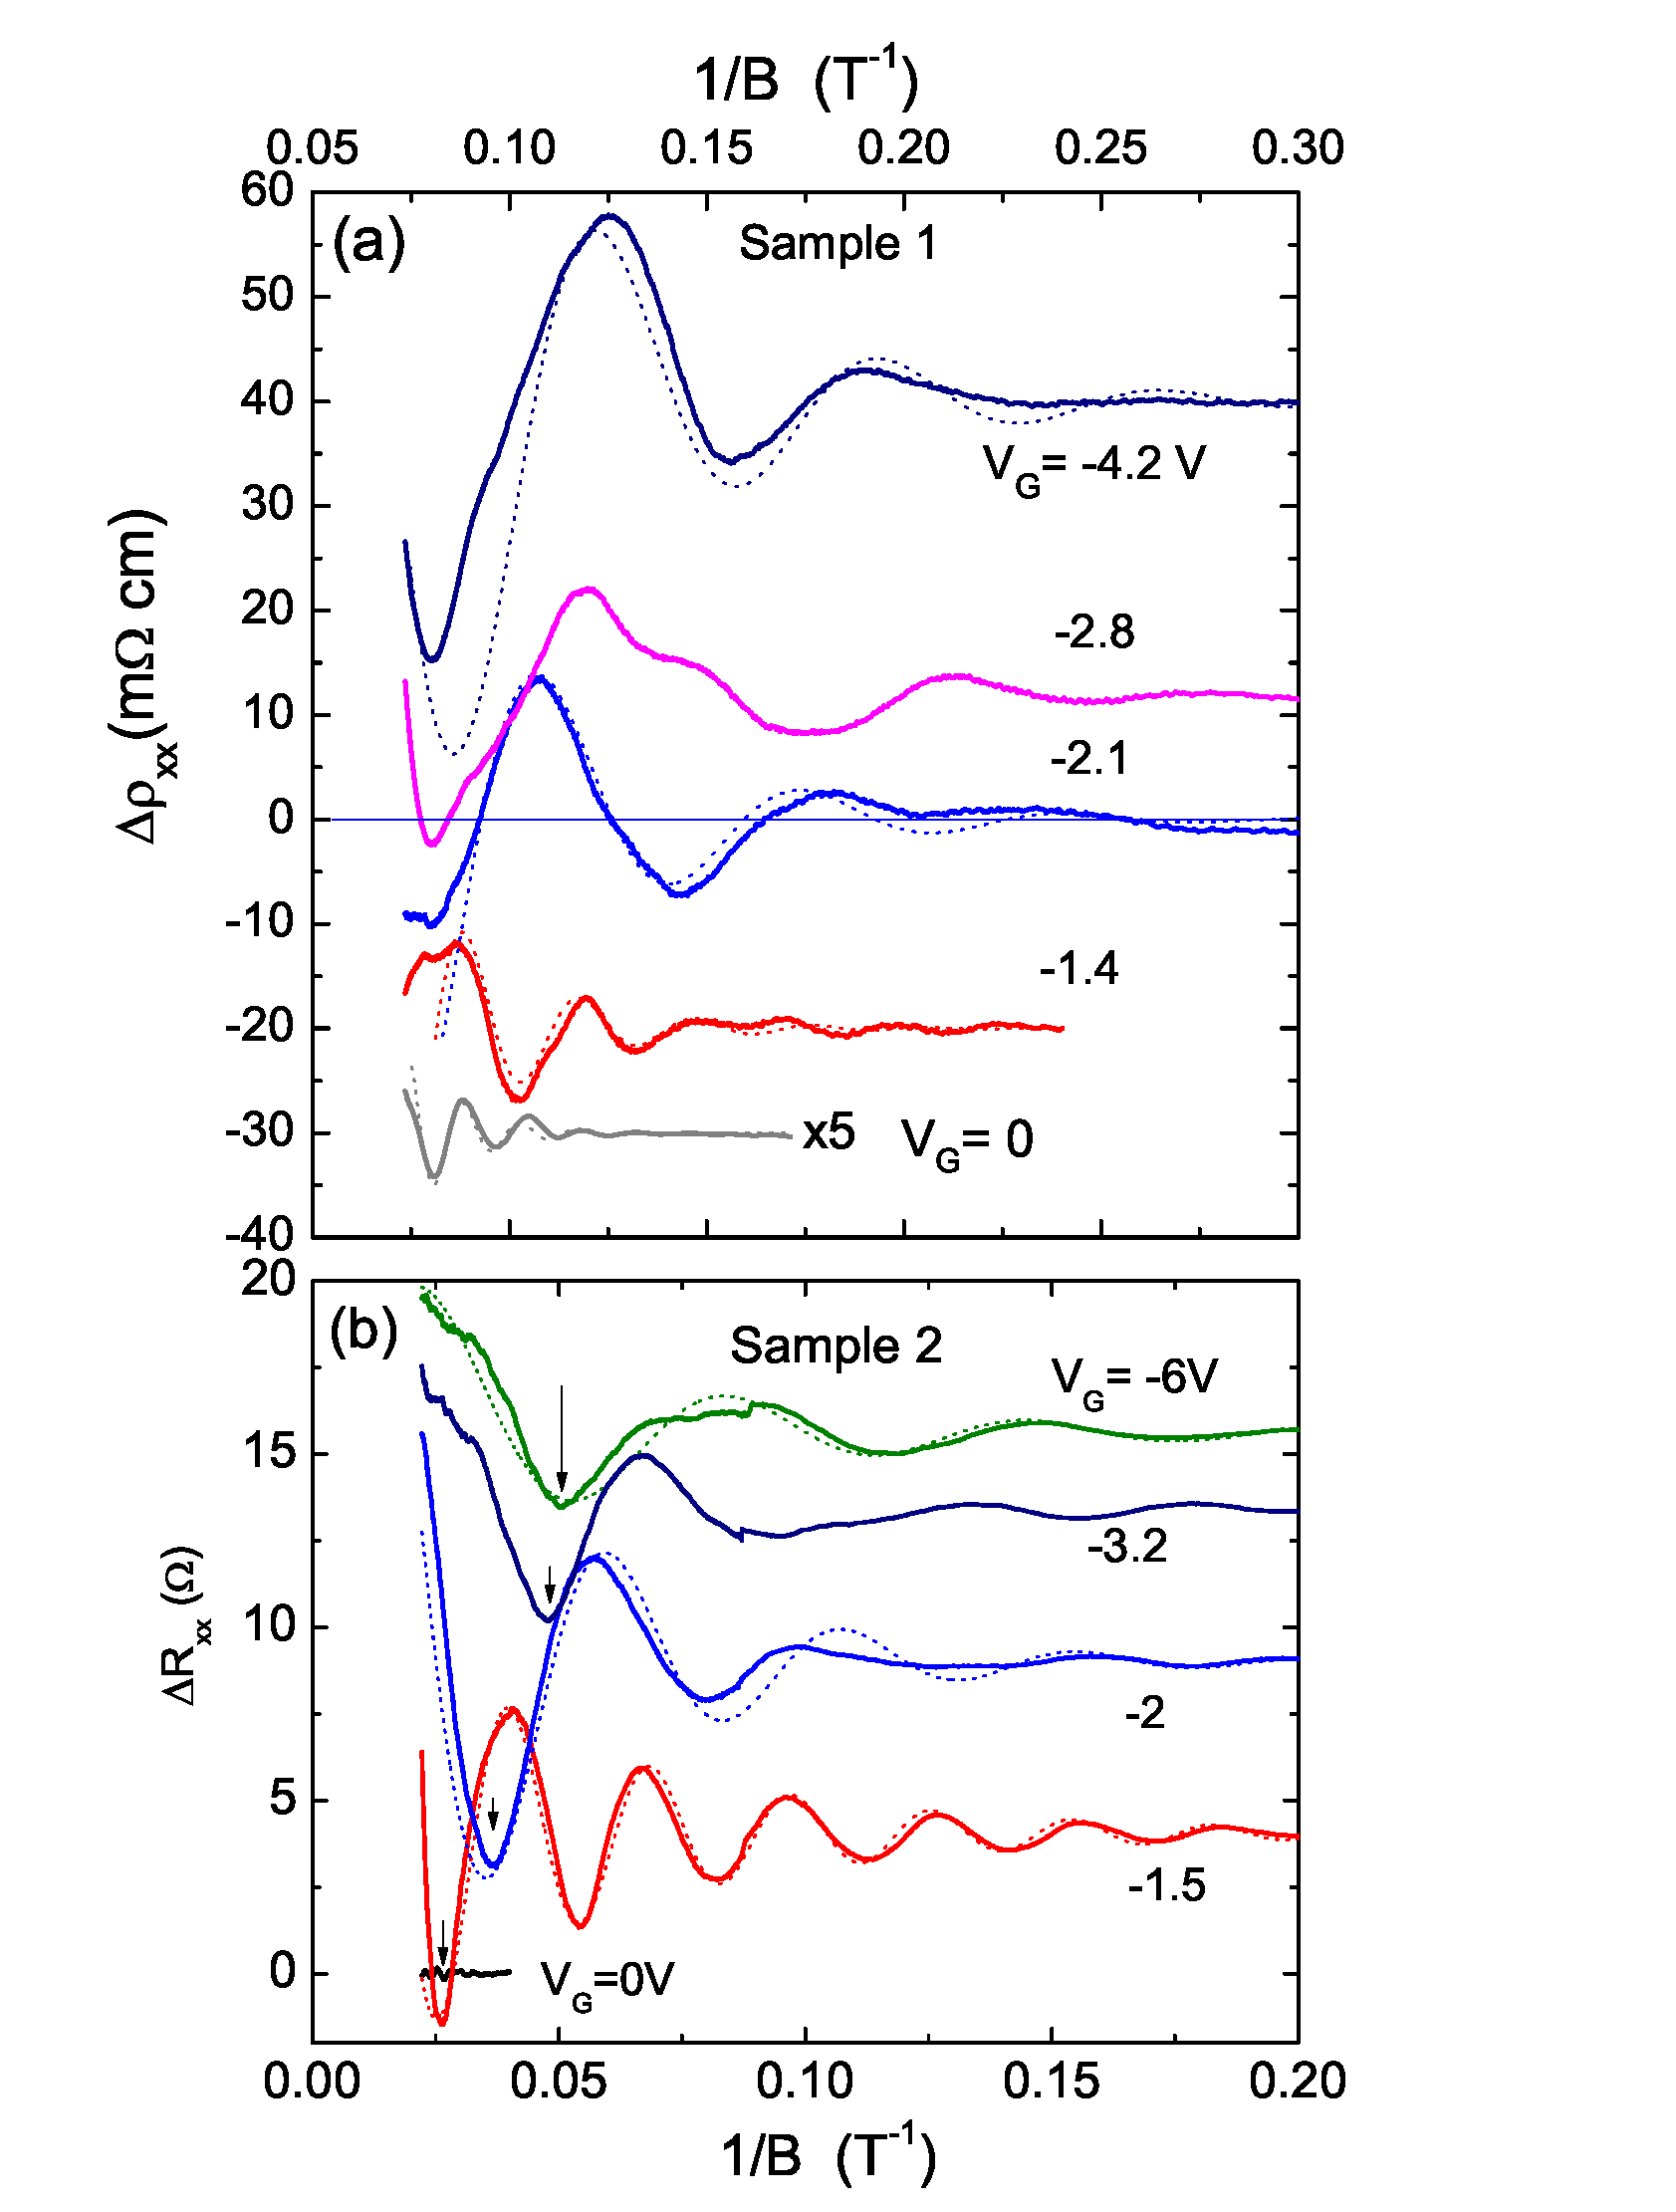
\includegraphics[width=0.85\linewidth]{ch-liquid/figures/FigSdHAll}
\caption{\label{figSdH_Vg}
Traces of SdH oscillations in the resistance versus $1/B$ curves of Sample 1 and 2,
showing systematic changes in the oscillation amplitudes and periods as the gate voltages increase
(bold curves, displaced vertically for clarity). The dashed curves
are fits to the LK expression with one frequency component~\cite{Xiong2012b}. 
Panel (a) shows traces of $\Delta\rho_{xx}$ 
vs. $1/B$ at 5 K measured up to 14 T for 5 values of $V_G$ (Sample 1). 
The largest increase in amplitudes occurs between $V_G$ = 0 V and -1.4 V. The curve
at $V_G = 0 V$ is shown after an amplification of $5\times$. All other curves share 
the same vertical scale. Panel (b) displays traces of $\Delta R_{xx}$ vs. $1/B$ at 0.3 K 
measured up to 45 T at $V_G$ as indicated (Sample 2).
Arrows indicate $n=\frac12$ ($E_F$ at center of broadened $N$ = 1 LL). 
}
  \end{center}
\end{figure} 

At each $V_G$, the magnetoresistance curves for both Sample 1 and 2 display giant SdH oscillations. In Fig. \ref{figSdH_Vg} we have subtracted a smooth background $\rho_B$ from the raw data to emphasize the SdH oscillatory part of the resistance. Therefore, the oscillatory part is $\Delta \rho_{xx} \equiv \rho_{xx} - \rho_{B}$, where $\rho_{B}$ is a smooth background. Fig. \ref{figSdH_Vg}a displays plots of $\Delta\rho_{xx}$ v.s. $1/B$ in Sample 1 for 5 different gate voltages. The period of the SdH oscillations clearly has a large monotonic increase as $V_G$ changes from 0 to -4.2 V, indicating a decreasing $E_F$ of the $n$-type surface states as we expected. Unexpectedly, the SdH amplitudes are strongly enhanced between $V_G = 0$ and -2.1 V (to show the former oscillations in the figure, we have amplified its amplitudes by 5$\times$). The dotted curves are the best fits ~\cite{Xiong2012b} to the Lifshitz-Kosevich (LK) expression for SdH oscillations using only one frequency component. From the fits, we can infer how the surface mobility $\mu_s$ changes with $V_G$ (see below). We find the same trend in Sample 2, which has a higher starting surface density $n_s$ but is taken to $B$ = 45 T (Fig. \ref{figSdH_Vg}b). Although the SdH oscillations are not resolved at $V_G=0$ V, they become prominent starting at $V_G$ = -1.5 V. From the fittings, we also notice that the steepest change in $\mu_s$ of Sample 2 occurs between $V_G$ = 0 and $V_G$ =$-$1.5V, at which $\mu_s$ =2800 $cm^2/(Vs)$. At a larger gating voltage, it saturates ($\mu_s$ = 3000 $cm^2/(Vs)$ at $-$6 V) as the gating effect saturates. 





%%%%%%%%%%%%%%%%%%%%%%%%%%%%%%%%%%
%%%%%%%%%%%%%%%%%%%%%%%%%%%%%%%%%%
%%%%%%%%%%%%%%%%%%%%%%%%%%%%%%%%%% FIGURE 3




%%%%%%%%%%%%%%%%%%%%%%%%%%%%%%%%%%
%%%%%%%%%%%%%%%%%%%%%%%%%%%%%%%%%%
%%%%%%%%%%%%%%%%%%%%%%%%%%%%%%%%%% FIGURE 4



